As described in \cref{sc: Theory}, the experiment is split up into two separate investigations. For each investigation, there is a change in the apparatus used to carry out the investigation. \\ 

For the first section of the investigation, a Thallium activated Sodium Iodide (denoted by NaI(Tl)) detector is used to measure the scattering electrons' energy. The detector contains two notable parts a NaI crystal and a photomultiplier tube (PMT). Once the crystal is activated by the presence of Thallium, it begins to produced scintillations by incident gamma rays which are then amplified by the PMT via a coupled photo-cathode. The scintillations are caused by the ionisation of sodium iodide, this allows for excited states within the crystal to decdecay-causinge 'flash'.\footnote{For more information on the technical details of how this works, please see Ref. \cite{an}} 

\begin{figure}[h!]
    \centering
    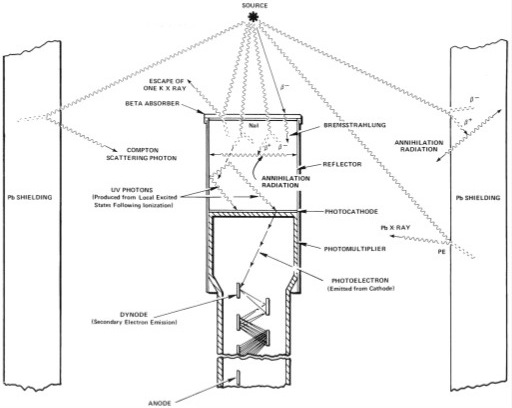
\includegraphics[width = 10cm]{Images/Nai.jpg}
    \caption{The structure of the NaI(Tl) detector and various types of gamma-ray interactions that occur in the typical source-detector-shield configuration \cite{an}}
\end{figure}

The photomultiplier used a high potential and the photoelectric effect to convert the scintillations to pulses. The pulses were then converted into an analogue signal; the signal was then outputted to a computer running a Maestro MCB25 software environment such that the gamma-ray spectrum was recorded. The programme allowed for counts, net-area and counting times to be determined. \\ 

For the second part of the experiment, the same software is used the NaI(Tl) detector, however, is swapped out for a Germanium, lithium doped detector (denoted by (Ge(Li))). The swap is that of accuracy the Ge(Li) detector will provide higher resolution. The higher resolution is provided from the presence of a doped semiconductor in the detector. The trade-off of using a semiconductor in the detector is noise, due to the presence of a doped semiconductor, there are impurities in the Ge, causing a lower energy threshold for electron-hold pairs is created. This is negated by having a depletion zone such that more considerable energies are needed to bridge and allow for current to flow\footnote{For a more detailed account of how the Ge(Li) detector operates, please see sections III and IV of Ref. \cite{rel_lab_manual} }.